\begin{tikzpicture}
\pgfdeclareplotmark{cross} {
\pgfpathmoveto{\pgfpoint{-0.3\pgfplotmarksize}{\pgfplotmarksize}}
\pgfpathlineto{\pgfpoint{+0.3\pgfplotmarksize}{\pgfplotmarksize}}
\pgfpathlineto{\pgfpoint{+0.3\pgfplotmarksize}{0.3\pgfplotmarksize}}
\pgfpathlineto{\pgfpoint{+1\pgfplotmarksize}{0.3\pgfplotmarksize}}
\pgfpathlineto{\pgfpoint{+1\pgfplotmarksize}{-0.3\pgfplotmarksize}}
\pgfpathlineto{\pgfpoint{+0.3\pgfplotmarksize}{-0.3\pgfplotmarksize}}
\pgfpathlineto{\pgfpoint{+0.3\pgfplotmarksize}{-1.\pgfplotmarksize}}
\pgfpathlineto{\pgfpoint{-0.3\pgfplotmarksize}{-1.\pgfplotmarksize}}
\pgfpathlineto{\pgfpoint{-0.3\pgfplotmarksize}{-0.3\pgfplotmarksize}}
\pgfpathlineto{\pgfpoint{-1.\pgfplotmarksize}{-0.3\pgfplotmarksize}}
\pgfpathlineto{\pgfpoint{-1.\pgfplotmarksize}{0.3\pgfplotmarksize}}
\pgfpathlineto{\pgfpoint{-0.3\pgfplotmarksize}{0.3\pgfplotmarksize}}
\pgfpathclose
\pgfusepathqstroke
}
\pgfdeclareplotmark{cross*} {
\pgfpathmoveto{\pgfpoint{-0.3\pgfplotmarksize}{\pgfplotmarksize}}
\pgfpathlineto{\pgfpoint{+0.3\pgfplotmarksize}{\pgfplotmarksize}}
\pgfpathlineto{\pgfpoint{+0.3\pgfplotmarksize}{0.3\pgfplotmarksize}}
\pgfpathlineto{\pgfpoint{+1\pgfplotmarksize}{0.3\pgfplotmarksize}}
\pgfpathlineto{\pgfpoint{+1\pgfplotmarksize}{-0.3\pgfplotmarksize}}
\pgfpathlineto{\pgfpoint{+0.3\pgfplotmarksize}{-0.3\pgfplotmarksize}}
\pgfpathlineto{\pgfpoint{+0.3\pgfplotmarksize}{-1.\pgfplotmarksize}}
\pgfpathlineto{\pgfpoint{-0.3\pgfplotmarksize}{-1.\pgfplotmarksize}}
\pgfpathlineto{\pgfpoint{-0.3\pgfplotmarksize}{-0.3\pgfplotmarksize}}
\pgfpathlineto{\pgfpoint{-1.\pgfplotmarksize}{-0.3\pgfplotmarksize}}
\pgfpathlineto{\pgfpoint{-1.\pgfplotmarksize}{0.3\pgfplotmarksize}}
\pgfpathlineto{\pgfpoint{-0.3\pgfplotmarksize}{0.3\pgfplotmarksize}}
\pgfpathclose
\pgfusepathqfillstroke
}
\pgfdeclareplotmark{newstar} {
\pgfpathmoveto{\pgfqpoint{0pt}{\pgfplotmarksize}}
\pgfpathlineto{\pgfqpointpolar{44}{0.5\pgfplotmarksize}}
\pgfpathlineto{\pgfqpointpolar{18}{\pgfplotmarksize}}
\pgfpathlineto{\pgfqpointpolar{-20}{0.5\pgfplotmarksize}}
\pgfpathlineto{\pgfqpointpolar{-54}{\pgfplotmarksize}}
\pgfpathlineto{\pgfqpointpolar{-90}{0.5\pgfplotmarksize}}
\pgfpathlineto{\pgfqpointpolar{234}{\pgfplotmarksize}}
\pgfpathlineto{\pgfqpointpolar{198}{0.5\pgfplotmarksize}}
\pgfpathlineto{\pgfqpointpolar{162}{\pgfplotmarksize}}
\pgfpathlineto{\pgfqpointpolar{134}{0.5\pgfplotmarksize}}
\pgfpathclose
\pgfusepathqstroke
}
\pgfdeclareplotmark{newstar*} {
\pgfpathmoveto{\pgfqpoint{0pt}{\pgfplotmarksize}}
\pgfpathlineto{\pgfqpointpolar{44}{0.5\pgfplotmarksize}}
\pgfpathlineto{\pgfqpointpolar{18}{\pgfplotmarksize}}
\pgfpathlineto{\pgfqpointpolar{-20}{0.5\pgfplotmarksize}}
\pgfpathlineto{\pgfqpointpolar{-54}{\pgfplotmarksize}}
\pgfpathlineto{\pgfqpointpolar{-90}{0.5\pgfplotmarksize}}
\pgfpathlineto{\pgfqpointpolar{234}{\pgfplotmarksize}}
\pgfpathlineto{\pgfqpointpolar{198}{0.5\pgfplotmarksize}}
\pgfpathlineto{\pgfqpointpolar{162}{\pgfplotmarksize}}
\pgfpathlineto{\pgfqpointpolar{134}{0.5\pgfplotmarksize}}
\pgfpathclose
\pgfusepathqfillstroke
}
\definecolor{c}{rgb}{1,1,1};
\draw [color=c, fill=c] (0,0) rectangle (20,14.3108);
\draw [color=c, fill=c] (2,1.43108) rectangle (18,12.8797);
\definecolor{c}{rgb}{0,0,0};
\draw [c,line width=0.9] (2,1.43108) -- (2,12.8797) -- (18,12.8797) -- (18,1.43108) -- (2,1.43108);
\definecolor{c}{rgb}{0.860294,0.872181,0.670343};
\draw [color=c, fill=c] (2,1.43108) rectangle (5.37553,3.57769);
\draw [color=c, fill=c] (5.37553,1.43108) rectangle (8.75105,3.57769);
\definecolor{c}{rgb}{0.664216,0.842157,0.861765};
\draw [color=c, fill=c] (8.75105,1.43108) rectangle (11.2489,3.57769);
\draw [color=c, fill=c] (12.2616,1.43108) rectangle (15.5021,3.57769);
\definecolor{c}{rgb}{0.482353,0.670588,0.894118};
\draw [color=c, fill=c] (15.5021,1.43108) rectangle (18,3.57769);
\definecolor{c}{rgb}{0.719608,0.263113,0.13652};
\draw [color=c, fill=c] (2,3.57769) rectangle (5.37553,5.00877);
\draw [color=c, fill=c] (5.37553,3.57769) rectangle (8.75105,5.00877);
\definecolor{c}{rgb}{0.864706,0.840686,0.58701};
\draw [color=c, fill=c] (8.75105,3.57769) rectangle (11.2489,5.00877);
\definecolor{c}{rgb}{0.860294,0.872181,0.670343};
\draw [color=c, fill=c] (12.2616,3.57769) rectangle (15.5021,5.00877);
\definecolor{c}{rgb}{0.600245,0.798039,0.875};
\draw [color=c, fill=c] (15.5021,3.57769) rectangle (18,5.00877);
\definecolor{c}{rgb}{0.823529,0.905882,0.823529};
\draw [color=c, fill=c] (2,5.00877) rectangle (5.37553,7.15539);
\draw [color=c, fill=c] (5.37553,5.00877) rectangle (8.75105,7.15539);
\definecolor{c}{rgb}{0.541299,0.734314,0.884559};
\draw [color=c, fill=c] (8.75105,5.00877) rectangle (11.2489,7.15539);
\draw [color=c, fill=c] (12.2616,5.00877) rectangle (15.5021,7.15539);
\definecolor{c}{rgb}{0.39951,0.584559,0.871814};
\draw [color=c, fill=c] (15.5021,5.00877) rectangle (18,7.15539);
\definecolor{c}{rgb}{0.18229,0.273751,0.887287};
\draw [color=c, fill=c] (2,7.15539) rectangle (5.37553,12.8797);
\draw [color=c, fill=c] (5.37553,7.15539) rectangle (8.75105,12.8797);
\draw [color=c, fill=c] (8.75105,7.15539) rectangle (11.2489,12.8797);
\draw [color=c, fill=c] (12.2616,7.15539) rectangle (15.5021,12.8797);
\draw [color=c, fill=c] (15.5021,7.15539) rectangle (18,12.8797);
\definecolor{c}{rgb}{0,0,0};
\draw (3.68776,2.50439) node[scale=1.39159, color=c, rotate=1]{$\genfrac{}{}{0pt}{}{3618535}{\pm 2088}$};
\draw (7.06329,2.50439) node[scale=1.39159, color=c, rotate=1]{$\genfrac{}{}{0pt}{}{3643834}{\pm 6358}$};
\draw (10,2.50439) node[scale=1.39159, color=c, rotate=1]{$\genfrac{}{}{0pt}{}{2189782}{\pm 9265}$};
\draw (13.8819,2.50439) node[scale=1.39159, color=c, rotate=1]{$\genfrac{}{}{0pt}{}{2334565}{\pm 4141}$};
\draw (16.7511,2.50439) node[scale=1.39159, color=c, rotate=1]{$\genfrac{}{}{0pt}{}{1535632}{\pm 2121}$};
\draw (3.68776,4.29323) node[scale=1.39159, color=c, rotate=1]{$\genfrac{}{}{0pt}{}{5893824}{\pm 1490}$};
\draw (7.06329,4.29323) node[scale=1.39159, color=c, rotate=1]{$\genfrac{}{}{0pt}{}{6189482}{\pm 3726}$};
\draw (10,4.29323) node[scale=1.39159, color=c, rotate=1]{$\genfrac{}{}{0pt}{}{3913823}{\pm 1794}$};
\draw (13.8819,4.29323) node[scale=1.39159, color=c, rotate=1]{$\genfrac{}{}{0pt}{}{3495316}{\pm 5733}$};
\draw (16.7511,4.29323) node[scale=1.39159, color=c, rotate=1]{$\genfrac{}{}{0pt}{}{1938728}{\pm 2224}$};
\draw (3.68776,6.08208) node[scale=1.39159, color=c, rotate=1]{$\genfrac{}{}{0pt}{}{2994426}{\pm 1835}$};
\draw (7.06329,6.08208) node[scale=1.39159, color=c, rotate=1]{$\genfrac{}{}{0pt}{}{2859425}{\pm 2587}$};
\draw (10,6.08208) node[scale=1.39159, color=c, rotate=1]{$\genfrac{}{}{0pt}{}{1833778}{\pm 2036}$};
\draw (13.8819,6.08208) node[scale=1.39159, color=c, rotate=1]{$\genfrac{}{}{0pt}{}{1832829}{\pm 3846}$};
\draw (16.7511,6.08208) node[scale=1.39159, color=c, rotate=1]{$\genfrac{}{}{0pt}{}{1001559}{\pm 1434}$};
\draw (3.68776,10.0175) node[scale=1.39159, color=c, rotate=1]{$\genfrac{}{}{0pt}{}{213076}{\pm 479}$};
\draw (7.06329,10.0175) node[scale=1.39159, color=c, rotate=1]{$\genfrac{}{}{0pt}{}{192060}{\pm 455}$};
\draw (10,10.0175) node[scale=1.39159, color=c, rotate=1]{$\genfrac{}{}{0pt}{}{115060}{\pm 354}$};
\draw (13.8819,10.0175) node[scale=1.39159, color=c, rotate=1]{$\genfrac{}{}{0pt}{}{118623}{\pm 359}$};
\draw (16.7511,10.0175) node[scale=1.39159, color=c, rotate=1]{$\genfrac{}{}{0pt}{}{61155}{\pm 257}$};
\draw [c,line width=0.9] (2,1.43108) -- (18,1.43108);
\draw [anchor=north] (3.68776,1.25935) node[scale=0.723624, color=c, rotate=0]{[0.0 - 0.5]};
\draw [anchor=north] (7.06329,1.25935) node[scale=0.723624, color=c, rotate=0]{[0.5 - 1.0]};
\draw [anchor=north] (10,1.25935) node[scale=0.723624, color=c, rotate=0]{[1.0 - 1.37]};
\draw [anchor=north] (13.8819,1.25935) node[scale=0.723624, color=c, rotate=0]{[1.52 - 2.0]};
\draw [anchor=north] (16.7511,1.25935) node[scale=0.723624, color=c, rotate=0]{[2.0 - 2.37]};
\draw [c,line width=0.9] (2,1.77454) -- (2,1.43108);
\draw [c,line width=0.9] (5.37553,1.77454) -- (5.37553,1.43108);
\draw [c,line width=0.9] (8.75105,1.77454) -- (8.75105,1.43108);
\draw [c,line width=0.9] (12.1266,1.77454) -- (12.1266,1.43108);
\draw [c,line width=0.9] (15.5021,1.77454) -- (15.5021,1.43108);
\draw [c,line width=0.9] (15.5021,1.77454) -- (15.5021,1.43108);
\draw [anchor= east] (18,0.309113) node[scale=1.11327, color=c, rotate=0]{$|\eta|_{  e}^{probe}$};
\draw [c,line width=0.9] (2,12.8797) -- (18,12.8797);
\draw [c,line width=0.9] (2,12.5362) -- (2,12.8797);
\draw [c,line width=0.9] (5.37553,12.5362) -- (5.37553,12.8797);
\draw [c,line width=0.9] (8.75105,12.5362) -- (8.75105,12.8797);
\draw [c,line width=0.9] (12.1266,12.5362) -- (12.1266,12.8797);
\draw [c,line width=0.9] (15.5021,12.5362) -- (15.5021,12.8797);
\draw [c,line width=0.9] (15.5021,12.5362) -- (15.5021,12.8797);
\draw [c,line width=0.9] (2,1.43108) -- (2,12.8797);
\draw [anchor= east] (1.76,2.50439) node[scale=0.723624, color=c, rotate=0]{[20 - 35] };
\draw [anchor= east] (1.76,4.29323) node[scale=0.723624, color=c, rotate=0]{[35 - 45] };
\draw [anchor= east] (1.76,6.08208) node[scale=0.723624, color=c, rotate=0]{[45 - 60] };
\draw [anchor= east] (1.76,10.0175) node[scale=0.723624, color=c, rotate=0]{[60 - 100]};
\draw [c,line width=0.9] (2.48,1.43108) -- (2,1.43108);
\draw [c,line width=0.9] (2.48,4.29323) -- (2,4.29323);
\draw [c,line width=0.9] (2.48,7.15539) -- (2,7.15539);
\draw [c,line width=0.9] (2.48,10.0175) -- (2,10.0175);
\draw [c,line width=0.9] (2.48,12.8797) -- (2,12.8797);
\draw [anchor= east] (0.432,12.8797) node[scale=1.11327, color=c, rotate=90]{$p_{T,  e}^{probe}  [GeV]$};
\draw [c,line width=0.9] (18,1.43108) -- (18,12.8797);
\draw [c,line width=0.9] (17.52,1.43108) -- (18,1.43108);
\draw [c,line width=0.9] (17.52,4.29323) -- (18,4.29323);
\draw [c,line width=0.9] (17.52,7.15539) -- (18,7.15539);
\draw [c,line width=0.9] (17.52,10.0175) -- (18,10.0175);
\draw [c,line width=0.9] (17.52,12.8797) -- (18,12.8797);
\definecolor{c}{rgb}{0.18229,0.273751,0.887287};
\draw [color=c, fill=c] (18.1,1.43108) rectangle (19,2.00351);
\definecolor{c}{rgb}{0.248071,0.40038,0.854396};
\draw [color=c, fill=c] (18.1,2.00351) rectangle (19,2.57594);
\definecolor{c}{rgb}{0.323039,0.505147,0.851225};
\draw [color=c, fill=c] (18.1,2.57594) rectangle (19,3.14837);
\definecolor{c}{rgb}{0.39951,0.584559,0.871814};
\draw [color=c, fill=c] (18.1,3.14837) rectangle (19,3.7208);
\definecolor{c}{rgb}{0.482353,0.670588,0.894118};
\draw [color=c, fill=c] (18.1,3.7208) rectangle (19,4.29323);
\definecolor{c}{rgb}{0.541299,0.734314,0.884559};
\draw [color=c, fill=c] (18.1,4.29323) rectangle (19,4.86566);
\definecolor{c}{rgb}{0.600245,0.798039,0.875};
\draw [color=c, fill=c] (18.1,4.86566) rectangle (19,5.4381);
\definecolor{c}{rgb}{0.664216,0.842157,0.861765};
\draw [color=c, fill=c] (18.1,5.4381) rectangle (19,6.01053);
\definecolor{c}{rgb}{0.743873,0.87402,0.842647};
\draw [color=c, fill=c] (18.1,6.01053) rectangle (19,6.58296);
\definecolor{c}{rgb}{0.823529,0.905882,0.823529};
\draw [color=c, fill=c] (18.1,6.58296) rectangle (19,7.15539);
\definecolor{c}{rgb}{0.842647,0.888358,0.743873};
\draw [color=c, fill=c] (18.1,7.15539) rectangle (19,7.72782);
\definecolor{c}{rgb}{0.860294,0.872181,0.670343};
\draw [color=c, fill=c] (18.1,7.72782) rectangle (19,8.30025);
\definecolor{c}{rgb}{0.864706,0.840686,0.58701};
\draw [color=c, fill=c] (18.1,8.30025) rectangle (19,8.87268);
\definecolor{c}{rgb}{0.851961,0.792892,0.499387};
\draw [color=c, fill=c] (18.1,8.87268) rectangle (19,9.44511);
\definecolor{c}{rgb}{0.839216,0.745098,0.411765};
\draw [color=c, fill=c] (18.1,9.44511) rectangle (19,10.0175);
\definecolor{c}{rgb}{0.817157,0.659804,0.345588};
\draw [color=c, fill=c] (18.1,10.0175) rectangle (19,10.59);
\definecolor{c}{rgb}{0.79326,0.567402,0.273897};
\draw [color=c, fill=c] (18.1,10.59) rectangle (19,11.1624);
\definecolor{c}{rgb}{0.768627,0.468382,0.216176};
\draw [color=c, fill=c] (18.1,11.1624) rectangle (19,11.7348);
\definecolor{c}{rgb}{0.743137,0.361642,0.174755};
\draw [color=c, fill=c] (18.1,11.7348) rectangle (19,12.3073);
\definecolor{c}{rgb}{0.719608,0.263113,0.13652};
\draw [color=c, fill=c] (18.1,12.3073) rectangle (19,12.8797);
\definecolor{c}{rgb}{0,0,0};
\draw [c,line width=0.9] (19,1.43108) -- (19,12.8797);
\draw [c,line width=0.9] (18.52,1.43108) -- (19,1.43108);
\draw [c,line width=0.9] (18.52,3.28077) -- (19,3.28077);
\draw [c,line width=0.9] (18.52,5.13046) -- (19,5.13046);
\draw [c,line width=0.9] (18.52,6.98015) -- (19,6.98015);
\draw [c,line width=0.9] (18.52,8.82984) -- (19,8.82984);
\draw [c,line width=0.9] (18.52,10.6795) -- (19,10.6795);
\draw [c,line width=0.9] (18.52,12.5292) -- (19,12.5292);
\draw [c,line width=0.9] (18.52,12.5292) -- (19,12.5292);
\draw [anchor= west] (19.1,1.43108) node[scale=1.11327, color=c, rotate=0]{0};
\draw [anchor= west] (19.1,3.28077) node[scale=1.11327, color=c, rotate=0]{1000};
\draw [anchor= west] (19.1,5.13046) node[scale=1.11327, color=c, rotate=0]{2000};
\draw [anchor= west] (19.1,6.98015) node[scale=1.11327, color=c, rotate=0]{3000};
\draw [anchor= west] (19.1,8.82984) node[scale=1.11327, color=c, rotate=0]{4000};
\draw [anchor= west] (19.1,10.6795) node[scale=1.11327, color=c, rotate=0]{5000};
\draw [anchor= west] (19.1,12.5292) node[scale=1.11327, color=c, rotate=0]{6000};
\draw [anchor=base west] (19,12.9298) node[scale=1.11327, color=c, rotate=0]{$\times10^{3}$};
\end{tikzpicture}
